\documentclass[../main.tex]{subfiles}
\begin{document}
\label{sec:ssloverview}
Before discussing previously proposed solutions to the problem we
identified in the Introdcution, we present here a generic overview of
SSL/TLS. In general, regardless of the cipher used, SSL/TLS utilises the
long-term private key to negotiate ephemeral keys for use in the
current session; hence, to secure the long-term private key, we need
to examine the session establishment mechanism. Roughly, SSL/TLS's
handshake can be split into four steps:

\begin{enumerate}
  \item \textbf{Contacting the server, and establishing parameters for
    the session}. Specifically, the exchange of hello messages that
    include: the server's certificate(s) a list of ciphers supported by
    each side (to determine which cipher is to be used for this session),
    \srandom, and \crandom. The random variables are used to derive the
    secret, used to secure communications.
  \item \textbf{Asymmetric key exchange}: based on the cipher
    selected, the client and server determine the asymmetric keys that are
    to be used to exchange the symmetric keys for the session. This step
    is necessary in two scenarios:
    \begin{enumerate}
      \item The client and server both possess public key
        certificates, and both entities wish to verify each other's identity
        during the handshake. We do not consider this case due to its
        rarity. Generally, the client verifies the server as part of the
        SSL/TLS handshake, and the server verifies the identity of the client
        via some other means, such as a username \& password.
      \item The client and server selected a cipher that offers
        forward secrecy. These ciphers function by first exchanging an
        ephemeral asymmetric secret. This secret is then used in negotiating
        the symmetric secret.
    \end{enumerate} In all other cases, the server's asymmetric keys
    are used to negotiate the ephemeral symmetric secret.
  \item \textbf{Ephemeral symmetric key negotiation}: The client and
    server establish the symmetric secret that is used for the current
    session. The symmetric ephemeral keys are calculated as outlined below:

    \begin{enumerate}
      \item The \crandom, \srandom, and a value denoted
        \texttt{PremasterSecret} are combined together, through use of a
        pseudo-random function (PRF), to generate a value called the
        \texttt{MasterSecret}. The \texttt{MasterSecret} is a 48-byte number,
        and is computed using the method outlined here in all SSL/TLS
        ciphers. In contrast, the \texttt{PremasterSecret} is a random value,
        established as part of this step. Arriving to the value of the
        \texttt{PremasterSecret}, however, depends on the cipher used.
      \item The \texttt{MasterSecret} is then used to generate a key block.
        A session key block consists of:
        \begin{itemize}
            \item \texttt{server_write_key}:
        \end{itemize}
    \end{enumerate}
    
    Calculating the symmetric secret is carried out through
    the following procedure:requires the random values
    exchanged in step 1 and a value denoted as the \texttt{PremasterSecret}.
    These three values are combined together through a pseudo-random function
    (PRF) to generate a value called the \texttt{MasterSecret}.
  \item \textbf{Verifying the integrity of the just-negotiated keys,
    completing the session establishment}: Both the server and the client
    compute a MAC across the packets exchanged in establishing the
    session. The resultant finished message is encrypted using the
    just-negotiated keys. If both sides successfully verify the MAC, the
    handshake is complete and the session is established. If either side
    fails to verify the MAC, the session is terminated.
\end{enumerate} Figure~\ref{fig:abshandshake} illustrates this
generalized SSL/TLS handshake.

\begin{figure}[H] \centering
  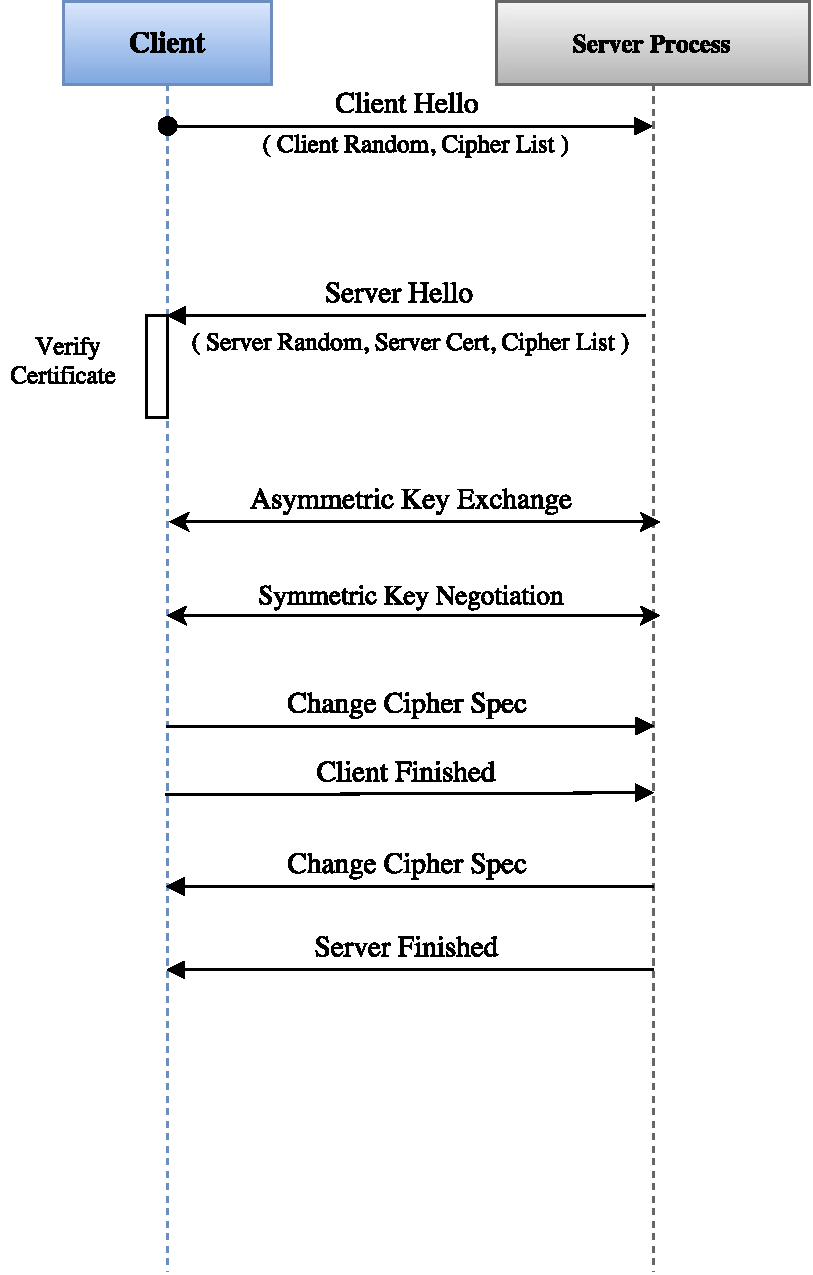
\includegraphics[scale=0.44]{images/abstract-handshake.pdf}
  \caption{SSL/TLS handshake generalization}
  \label{fig:abshandshake}
\end{figure}

\end{document}